\section{Auswertung}
\label{sec:auswertung}

\subsection{Charakteristik des Zählrohres}
\label{subsec:charakteristik}

In Inkrementen von $10 \,\unit{\volt}$ wird die Spannung von $350 \,\unit{\volt}$ auf $700 \,\unit{\volt}$ erhöht.
Zu jeder Spannung $U$ wird dabei über einen Zeitraum von zwei Minuten die Teilchenzahl $N$ aufgenommen, die aufgenommenen Messdaten sind dabei in \autoref{tab:messung1} dargestellt.

\begin{table}[H]
    \centering
    \caption{Eintreffende Teilchenzahl $N$ in Abhängigkeit der Spannung $U$.}
    \label{tab:messung1}
    \begin{tabular}{S[table-format=3.0] S[table-format=5.0]}
      \toprule
        {$U \mathbin{/} \unit{\volt}$} & {$N$ in $120 \,\unit{\second}$} \\
      \midrule
        350         &           14737           \\
        360         &           14534           \\
        370         &           14835           \\
        380         &           14881           \\
        390         &           14749           \\
        400         &           14886           \\        
        410         &           14693           \\
        420         &           14795           \\
        430         &           14700           \\
        440         &           15023           \\
        450         &           14809           \\
        460         &           14631           \\
        470         &           14935           \\
        480         &           14865           \\
        490         &           14850           \\
        500         &           14921           \\
        510         &           14625           \\
        520         &           14925           \\
        530         &           14841           \\
        540         &           14801           \\
        550         &           14948           \\
        560         &           15026           \\
        570         &           15122           \\
        580         &           14837           \\
        590         &           15194           \\
        600         &           15043           \\
        610         &           15280           \\
        620         &           15134           \\
        630         &           15255           \\
        640         &           14959           \\
        650         &           15296           \\
        660         &           15403           \\
        670         &           15574           \\
        680         &           15498           \\
        690         &           15729           \\
        700         &           15689           \\
    \bottomrule
    \end{tabular}
\end{table}

Das Plateau kann dabei zwischen ungefähr $400 \,\unit{\volt}$ und $600 \,\unit{\volt}$ angenommen werden.
Die durchgeführte lineare Ausgleichsrechnung der Form

\begin{equation*}
      y = m x + n
\end{equation*}

besitzt dabei die Koeffizienten

\begin{equation*}
      m = 0.8466 \pm ...
\end{equation*}

sowie

\begin{equation*}
      n = 14433.4150 \pm ... \,.
\end{equation*}

Der dazugehörige Graph mitsamt Ausgleichsgerade ist dabei in \autoref{fig:graph1} dargestellt.

\begin{figure}
    \centering
    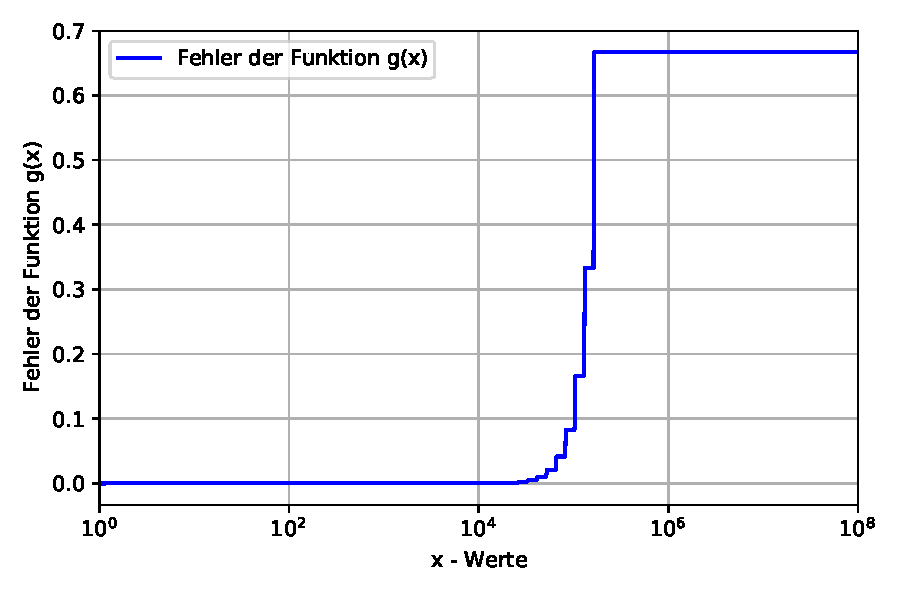
\includegraphics{build/Graph_b.pdf}
    \caption{Aufgenommene Teilchenzahl $N$ in Spannungsabhängig sowie durchgeführte Ausgleichsrechnung.}
    \label{fig:graph1}
\end{figure}


\subsection{Nachentladungen}

Die Spannung am Zählrohr wird zunächst so weit heruntergeregelt, dass am Oszilloskop kein zweiter hervorgerufener Impuls sichtbar ist.
Nachdem die Spannung auf $700 \,\unit{\volt}$ erhöht wird, sind auf dem Oszilloskop weitere Impulse sichtbar, die Nachentladungen.
Mithilfe von \autoref{fig:messung2} bestimmt sich der Abstand zwischen Primär- und Nachentladung dabei zu ungefähr $200 \,\unit{\micro\second}$.

\begin{figure}
    \centering
    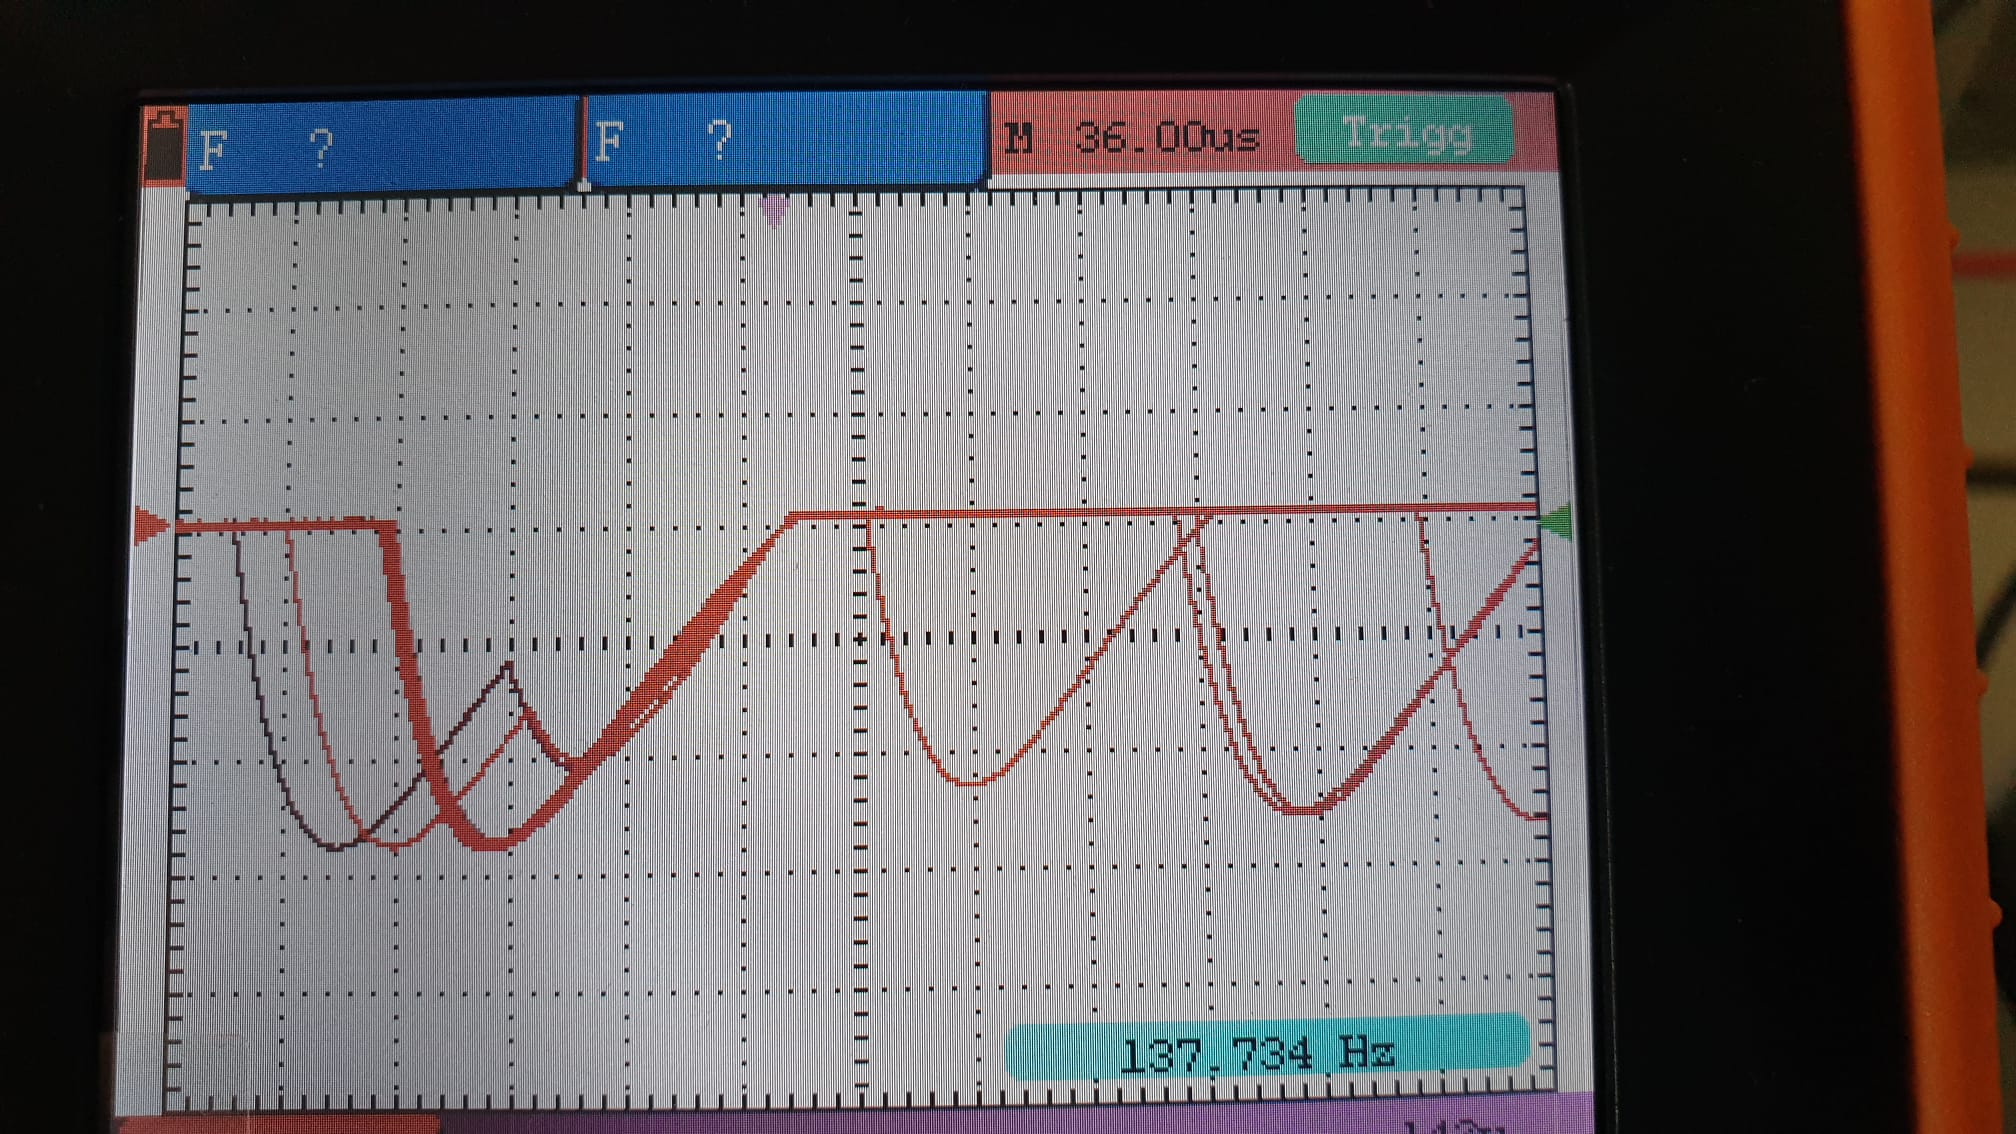
\includegraphics[scale=0.2]{figures/messung2.jpeg}
    \caption{Primär- und Nachentladungen bei $U = 700 \,\unit{\volt}$ bei $50 \,\unit{\micro\second}$ pro Kästchen.}
    \label{fig:messung2}
\end{figure}


\subsection{Bestimmung der Totzeit}

Aus \autoref{fig:messung2} lässt sich neben dem Abstand zwischen Primär- und Nachentladungen auch die Totzeit ablesen.
Die beträgt dabei ungefähr
\begin{equation*}
    T \approx 75 \,\unit{\micro\second} \,.
\end{equation*}

Genauer kann sie jedoch über die Zwei-Quellen-Methode bestimmt werden.
In \autoref{tab:messung3} sind dabei die Teilchenzahlen der beiden Einzelquellen sowie beider Quellen gemeinsam, erneut auf einem Intervall von $120 \,\unit{\second}$ mitsamt der nach \eqref{eq:totzeit} berechneten Totzeit dargestellt.

\begin{table}[H]
    \centering
    \caption{Teilchenzahlen der Quellen sowie Totzeit $T$.}
    \label{tab:messung3}
    \begin{tabular}{|S | S|}
      \hline
        {$N_1$}                             &  22084    \\
        \hline
        {$N_{1 + 2}$ }                      &  40352    \\
        \hline
        {$N_2$}                             &  18864    \\
        \hline
        {$T \mathbin{/} \unit{\second}$}    &  {$7,1533 \cdot 10^{-07}$} \\
    \hline
    \end{tabular}
\end{table}


\subsection{Freigesetzte Ladung pro Teilchen}
\label{subsec:ladung}

Mithilfe des bereits bei der zu \autoref{subsec:charakteristik} gehörigen Messung aufgenommenen Stroms und \eqref{eq:teilchenstrom} wird die freigesetzte Ladung $\Delta Q$ berechnet.
In \autoref{tab:messung4} sind dabei die Spannungen, Ströme, sowie die freigesetzten Ladungen, diese jeweils in $\unit{\coulomb}$ sowie in Elementarladungen $\text{e}$ aufgetragen.

\begin{table}[H]
    \centering
    \caption{Eintreffende Teilchenzahl $N$ in Abhängigkeit der Spannung $U$.}
    \label{tab:messung4}
    \begin{tabular}{S[table-format=3.0] S[table-format=1.3] S  S}
      \toprule
        {$U \mathbin{/} \unit{\volt}$} & {$I \mathbin{/} \unit{\micro\ampere}$} & {$\Delta Q \mathbin{/} \unit{\coulomb}$} & {$\frac{\Delta Q}{\text{e}}$} \\
      \midrule
      350            &         0.200        &       {$1,6286 \cdot 10^{-9}$}        &       {$1,0165 \cdot 10^{10}$}       \\
      360            &         0.150        &       {$1,2385 \cdot 10^{-9}$}        &       {$7,7300 \cdot 10^{9}$}       \\
      370            &         0.175        &       {$1,4156 \cdot 10^{-9}$}        &       {$8,8353 \cdot 10^{9}$}       \\
      380            &         0.200        &       {$1,6128 \cdot 10^{-9}$}        &       {$1,0066 \cdot 10^{10}$}       \\
      390            &         0.200        &       {$1,6272 \cdot 10^{-9}$}        &       {$1,0156 \cdot 10^{10}$}       \\
      400            &         0.220        &       {$1,7735 \cdot 10^{-9}$}        &       {$1,1069 \cdot 10^{10}$}       \\
      410            &         0.220        &       {$1,7968 \cdot 10^{-9}$}        &       {$1,1215 \cdot 10^{10}$}       \\
      420            &         0.250        &       {$2,0277 \cdot 10^{-9}$}        &       {$1,2656 \cdot 10^{10}$}       \\
      430            &         0.300        &       {$2,4490 \cdot 10^{-9}$}        &       {$1,5285 \cdot 10^{10}$}       \\
      440            &         0.350        &       {$2,7957 \cdot 10^{-9}$}        &       {$1,7450 \cdot 10^{10}$}       \\
      450            &         0.360        &       {$2,9172 \cdot 10^{-9}$}        &       {$1,8207 \cdot 10^{10}$}       \\
      460            &         0.380        &       {$3,1167 \cdot 10^{-9}$}        &       {$1,9453 \cdot 10^{10}$}       \\
      470            &         0.380        &       {$3,0532 \cdot 10^{-9}$}        &       {$1,9057 \cdot 10^{10}$}       \\
      480            &         0.400        &       {$3,2291 \cdot 10^{-9}$}        &       {$2,0154 \cdot 10^{10}$}       \\
      490            &         0.400        &       {$3,2323 \cdot 10^{-9}$}        &       {$2,0175 \cdot 10^{10}$}       \\
      500            &         0.410        &       {$3,2974 \cdot 10^{-9}$}        &       {$2,0581 \cdot 10^{10}$}       \\
      510            &         0.400        &       {$3,2821 \cdot 10^{-9}$}        &       {$2,0485 \cdot 10^{10}$}       \\
      520            &         0.450        &       {$3,6181 \cdot 10^{-9}$}        &       {$2,2582 \cdot 10^{10}$}       \\
      530            &         0.500        &       {$4,0429 \cdot 10^{-9}$}        &       {$2,5234 \cdot 10^{10}$}       \\
      540            &         0.500        &       {$4,0538 \cdot 10^{-9}$}        &       {$2,5302 \cdot 10^{10}$}       \\
      550            &         0.500        &       {$4,0139 \cdot 10^{-9}$}        &       {$2,5053 \cdot 10^{10}$}       \\
      560            &         0.500        &       {$3,9931 \cdot 10^{-9}$}        &       {$2,4923 \cdot 10^{10}$}       \\
      570            &         0.500        &       {$3,9677 \cdot 10^{-9}$}        &       {$2,4765 \cdot 10^{10}$}       \\
      580            &         0.580        &       {$4,6910 \cdot 10^{-9}$}        &       {$2,9279 \cdot 10^{10}$}       \\
      590            &         0.600        &       {$4,7387 \cdot 10^{-9}$}        &       {$2,9577 \cdot 10^{10}$}       \\
      600            &         0.600        &       {$4,7862 \cdot 10^{-9}$}        &       {$2,9874 \cdot 10^{10}$}       \\
      610            &         0.600        &       {$4,7120 \cdot 10^{-9}$}        &       {$2,9410 \cdot 10^{10}$}       \\
      620            &         0.600        &       {$4,7575 \cdot 10^{-9}$}        &       {$2,9694 \cdot 10^{10}$}       \\
      630            &         0.620        &       {$4,8771 \cdot 10^{-9}$}        &       {$3,0440 \cdot 10^{10}$}       \\
      640            &         0.600        &       {$4,8132 \cdot 10^{-9}$}        &       {$3,0041 \cdot 10^{10}$}       \\
      650            &         0.600        &       {$4,7071 \cdot 10^{-9}$}        &       {$2,9380 \cdot 10^{10}$}       \\
      660            &         0.600        &       {$4,6745 \cdot 10^{-9}$}        &       {$2,9175 \cdot 10^{10}$}       \\
      670            &         0.600        &       {$4,6231 \cdot 10^{-9}$}        &       {$2,8855 \cdot 10^{10}$}       \\
      680            &         0.700        &       {$5,4201 \cdot 10^{-9}$}        &       {$3,3829 \cdot 10^{10}$}       \\
      690            &         0.800        &       {$6,1034 \cdot 10^{-9}$}        &       {$3,8094 \cdot 10^{10}$}       \\
      700            &         0.750        &       {$5,7365 \cdot 10^{-9}$}        &       {$3,5804 \cdot 10^{10}$}       \\ 
    \bottomrule
    \end{tabular}
\end{table}
